\documentclass[landscape,10pt]{article}
\usepackage[latin1]{inputenc}

\usepackage{ae}
\usepackage{amssymb}
\usepackage{url}
\usepackage{xspace}

\usepackage{tikz}
\usetikzlibrary{mindmap,trees}
\usetikzlibrary{shapes}

% set up externalization
\usetikzlibrary{external}
\tikzset{external/system call={latex \tikzexternalcheckshellescape -halt-on-error
-interaction=batchmode -jobname "\image" "\texsource";
dvips -o "\image".ps "\image".dvi;
ps2eps "\image.ps"}}
\tikzexternalize

%% https://www.bu.edu/math/files/2013/08/tikzpgfmanual.pdf

\begin{document}

\tikzstyle{root concept}+=[concept color=red!60]
%% \tikzstyle{level 1 concept}+=[set style={{every child}=[concept color=orange!50]}]
%% \tikzstyle{level 2 concept}+=[set style={{every child}=[concept color=blue!20]}]


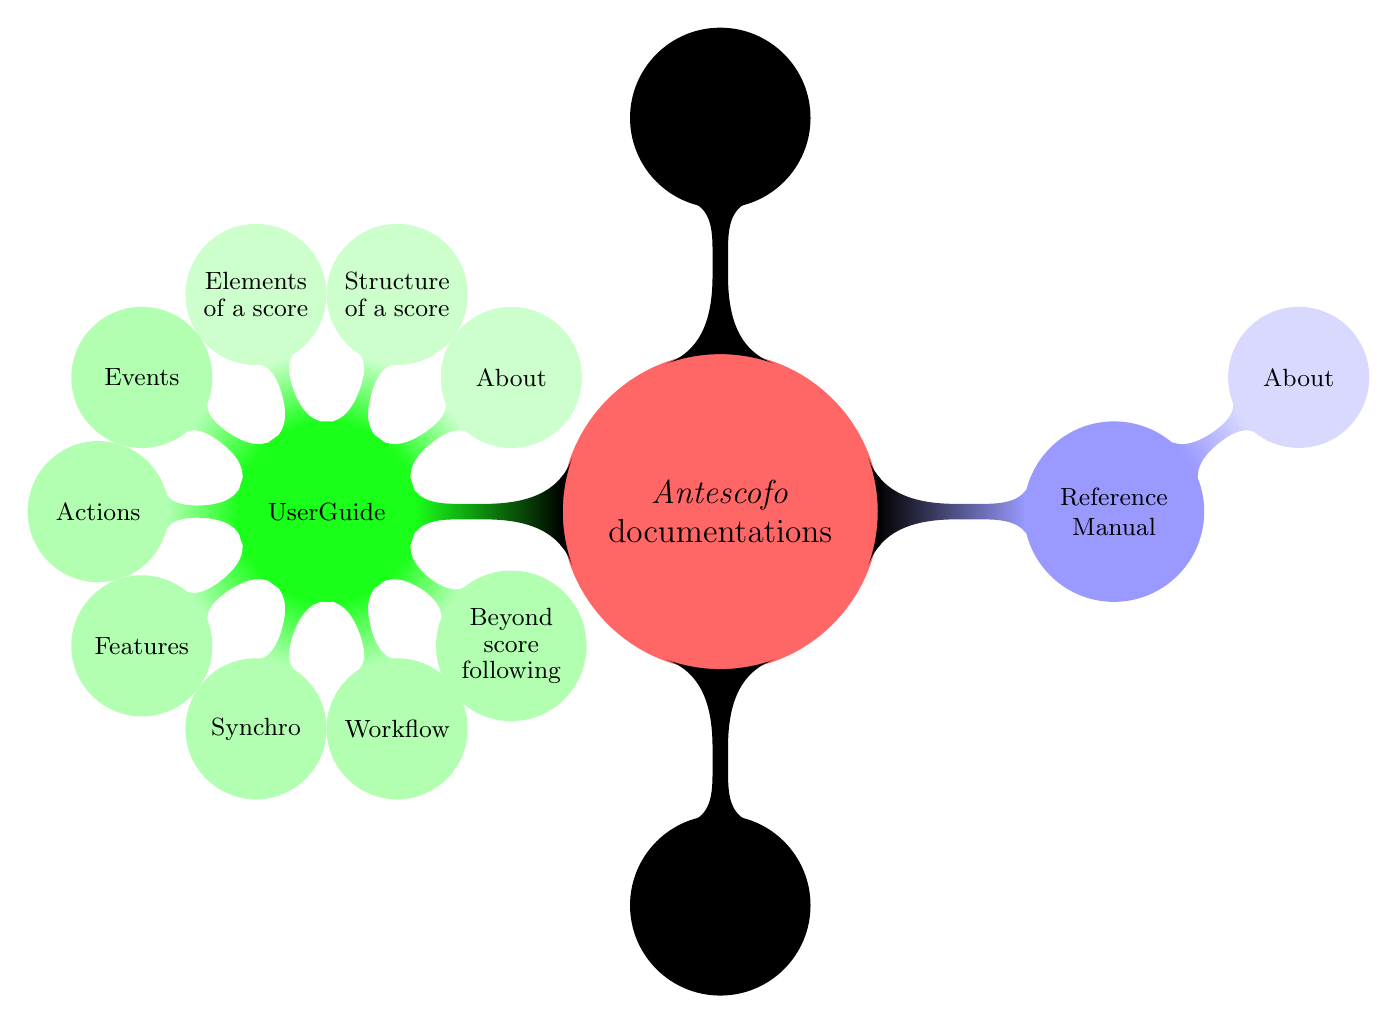
\begin{tikzpicture}[mindmap, level distance=30mm]

      \node[concept, concept color=red!60] {\emph{Antescofo}\\ documentations}
      %% 
      child[grow=180, concept color=green!90]
      {
        node[concept] {UserGuide}
        child[grow=36, concept color=green!20]  {node [concept] {\small About}}
        child[grow=72, concept color=green!20]  {node [concept] {\small Structure of a score}}
        child[grow=108, concept color=green!20] {node [concept] {\small Elements of a score}}
        child[grow=144, concept color=green!30] {node [concept] {\small Events}}
        child[grow=180, concept color=green!30] {node [concept] {\small Actions}}
        child[grow=216, concept color=green!30] {node [concept] {\small Features}}
        child[grow=252, concept color=green!30] {node [concept] {\small Synchro}}
        child[grow=288, concept color=green!30] {node [concept] {\small Workflow}}
        child[grow=324, concept color=green!30] {node [concept] {\small Beyond score following}}
      }
      %%
      child[grow=0, concept color=blue!40] 
      {
        node[concept] {Reference Manual}
        child[grow=36, concept color=blue!15]  {node [concept] {\small About}}
      }
    child[grow=90] 
    {
      node[concept] {Library Manual}
    }
    child[grow=-90] 
    {
      node[concept] {How To}
    };

\end{tikzpicture}




\end{document}
